\chapter{Métodos de Sincronismo}
\label{Ch:3}
\graphicspath{{figs/}}
\section{Sincronismo en OFDM}
\label{S:ch3-sincronismo}

\subsection{Sincronismo en Tiempo}
\label{Ss:ch3-sincronismo-tiempo}

La transmisión OFDM, tal como fue vista en el capítulo \ref{Ch:2}, consiste en el envío consecutivo de símbolos OFDM, construídos por una operación IFFT y la aplicación de un intervalo de guarda. Para recuperar los valores asignados a las subportadoras, el receptor debe aplicar una operación FFT al intervalo correcto. Por este motivo este tiene que ser capaz de identificar el instante en el que cada símbolo OFDM inicia.

En un canal real, puede existir una respuesta al impulso finita que contamine las muestras pertenecientes a símbolos siguientes con las muestras pertenecientes al símbolo actual. El intervalo de guarda cumple la función de permitir que la respuesta al impulso del canal se extinga antes de la ventana FFT que aplicará el receptor.

La interferencia inter-símbolos (ISI por sus siglas en inglés) en OFDM existe cuando la ventana FFT aplicada por el receptor se desvía respecto a la ideal. Si esta se adelanta se produce ISI con el símbolo siguiente, mientras que si se atrasa se produce ISI con el símbolo anterior.\\
\begin{figure}[ht]
    \centering{}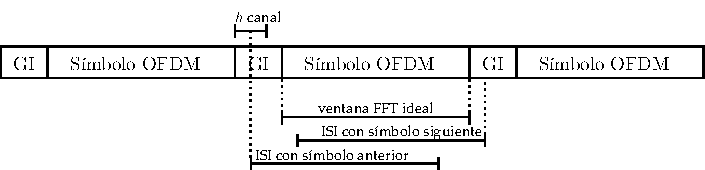
\includegraphics[width=\imsizeL ]{ventana-fft.pdf}
    \caption{Secuencia de entrenamiento de símbolos cortos en el dominio temporal.\label{fig:ventana-fft}}  
\end{figure}

El sincronismo en tiempo requiere entonces identificar precisamente el instante en el que inició la recepción de una PPDU, así como conocer la longitud de los símbolos OFDM. En este capítulo se definen métodos para identificar la muestra precisa en la que la transmisión inicia utilizando la secuencia de entrenamiento de símbolos cortos definida en el capítulo \ref{Ch:2}.

\subsection{Sincronismo en Frecuencia}
\label{Ss:ch3-sincronismo-frecuencia}

Se supone que una señal $x[n]$ generada en un transmisor en banda base y transmitida a través de un canal. La señal $x(t)$ llega a un receptor. La señal contiene un componente en fase y en cuadratura. 
\begin{equation}
    x(t) = x_I(t)\cos(2\pi f_c t) + x_Q(t)\sin(2\pi f_c t)
\end{equation}

La frecuencia de portadora, $f_c$, es aquella tal que al demodular y muestrear $x(t)$ con un demodulador coherente tal como el que se observa en la figura \ref{fig:demod-err} se obtiendría exáctamente $x[n]$.

\begin{figure}[ht]
    \centering{}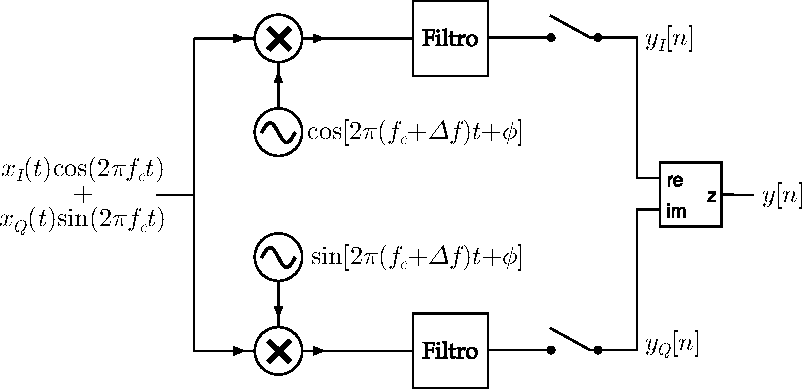
\includegraphics[width=\imsize]{demod-err.pdf}
    \caption{Secuencia de entrenamiento de símbolos cortos en el dominio temporal.\label{fig:demod-err}}  
\end{figure}

Sin embargo, el receptor desconoce $f_c$, sino que demodula la señal con un oscilador local que tiene una frecuencia propia, expresada como $f_c+\Delta f$ en donde $\Delta f$ es el error de frecuencia, y contempla impresiciones en los osciladores locales del receptor y transmisor, así como efectos Doppler que pueden estar presentes en el canal.

Además, se desconoce la fase con la que llega la señal, $\phi$, provocada por el camino óptico entre transmisor y receptor.

Al demodular y muestrear la señal, se obtiene la señal $y[n]$, la cual una vez afectada por los errores en fase y en frecuencia será.\\
\begin{equation}
    y[n] = x[n] e^{j(2\pi\Delta f T_s n + \phi)}
\end{equation}


\section{Banco de Correladores}
\label{S:ch3-banco}

Definiciones principales: la señal recibida lleva el nombre de $\mathbf{y}$, la secuencia de entrenamiento de símbolos cortos es conocida y lleva el nombre de $\mathbf{s}$, y tiene una longitud de $N$ muestras.

\subsection{Estimación con una única referencia}

Suponemos que se desea sincronizar en tiempo y no existe error en frecuencia. Únicamente se desea una función que sea máxima al inicio del preámbulo. Una forma intuitiva de diseñar esa función es calculando la correlación de las últimas $N$ muestras de la señal recibida con el preámbulo, el cual es conocido por el receptor.
\begin{equation}\label{eq:correladores-1}
    \Phi[n] = \left\lvert \sum_{k=1}^{N}y^\ast[n-k]s[N-k] \right\rvert
\end{equation}

Considerando la ecuación \ref{eq:correladores-1}, es fácil ver que $\Phi$ es máxima en el caso que las últimas $N$ muestras recibidas son exáctamente las muestras de $\mathbf{s}$, eventualmente modificadas por un factor de escala complejo, y que su valor es\\
\begin{equation}\label{eq:correladores-2}
    y[n-k] = As[N-k] \quad \rightarrow \quad \Phi = A \lVert \mathbf{s} \rVert
\end{equation}

Se observa que el error en fase no afecta la estimación del instante inicial de recepción.

\begin{figure}[ht]
    \centering{}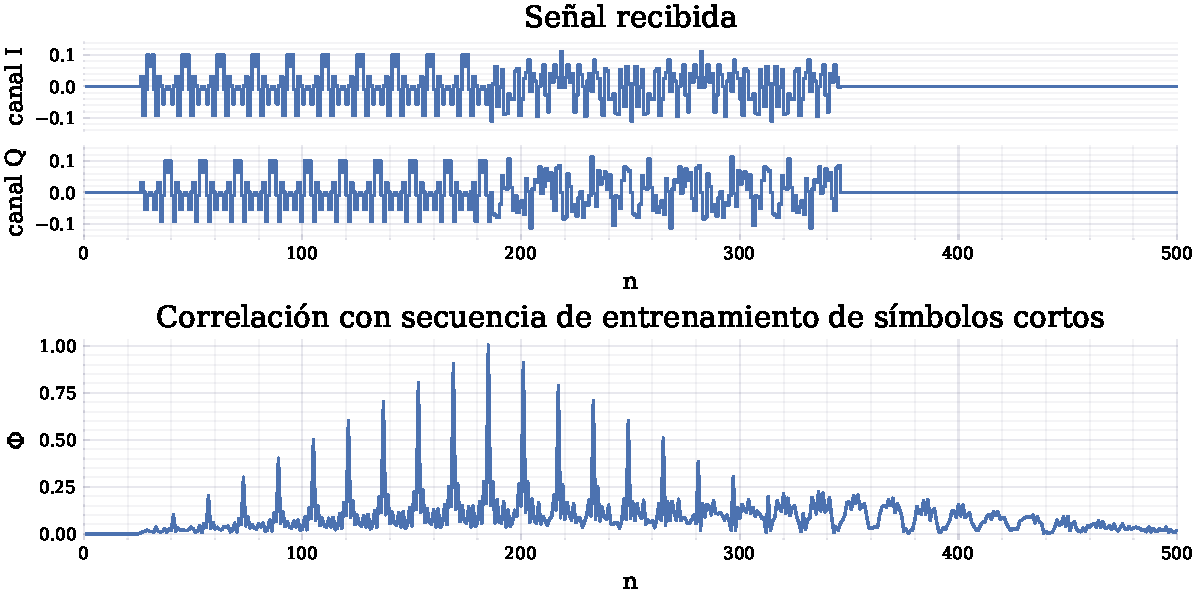
\includegraphics[width=\imsizeL]{banco-xcorr1.pdf}
    \caption{Secuencia de entrenamiento de símbolos cortos en el dominio temporal.\label{fig:banco-xcorr1}}  
\end{figure}


\subsection{Estimación de error en frecuencia}
\label{Ss:ch3-banco-frecuencias}
El método de correlación con la secuencia de entrenamiento de símbolos cortos tal como fue definido es capaz de iniciar el sincronismo en tiempo, pero aún no es capaz de inicializar sincronismo en frecuencia. Efectivamente se demostró que un error en fase no afecta, pero si existe un error de frecuencia se degrada el valor del estimador. 

Esta degradación se puede calcular definiendo el factor de rotación de fase
\begin{equation}
    \text{Factor de rotación de fase} = \Delta f T_s
\end{equation}

Asimismo se define el factor de degradación
\begin{equation}
    \text{Factor de degradacíon} = \frac{\Phi_{Max}(\Delta f)}{\Phi_{Max}\lvert_{\Delta f = 0}}
\end{equation}

El factor de degradación en función del factor de rotación de fase se calcula numéricamente y se grafica en la figura \ref{fig:degradacion}.\\
\begin{figure}[ht]
    \centering{}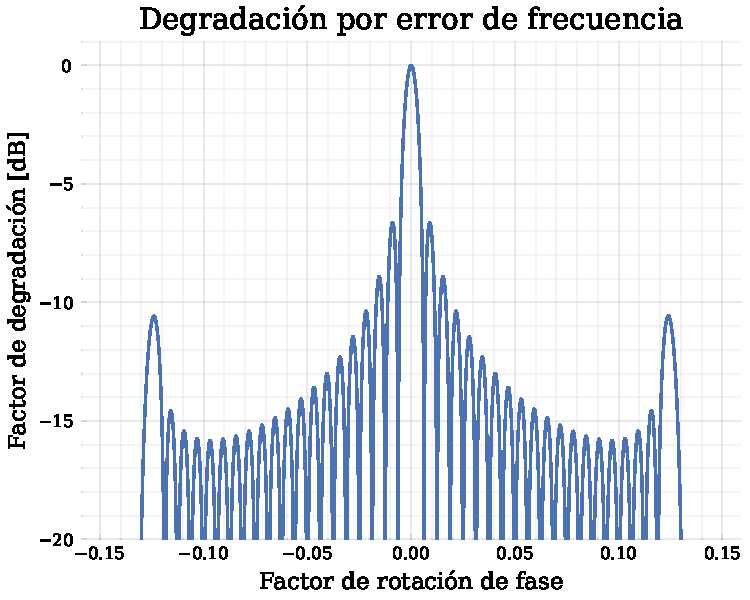
\includegraphics[width=\imsize]{degradacion-err-freq.pdf}
    \caption{Secuencia de entrenamiento de símbolos cortos en el dominio temporal.\label{fig:degradacion}}  
\end{figure}

En particular, el factor de degradación alcanza -3 dB para factores de rotación de fase de $\Delta f T_s = \pm 0.0037$.

El principio utilizado para la estimación con un único correlador se puede utilizar para extender el método. Suponemos que se elige un rango de $M$ valores que puede tomar $\Delta f$. Es posible, para cada valor, generar una referencia del preámbulo con la rotación lineal en fase correspondiente a ese error en frecuencia.\\
\begin{equation}
    s_m[k] = s[k] e^{j2\pi \frac{m\Delta f}{M} T_s k}
\end{equation}

El criterio de factor de rotación en fase se puede utilizar para elegir el espaciamiento entre frecuencias para las múltiples referencias. Algunas de las referencias creados usando este criterio se visualizan en la figura \ref{fig:references}.\\
\begin{figure}[ht]
    \centering{}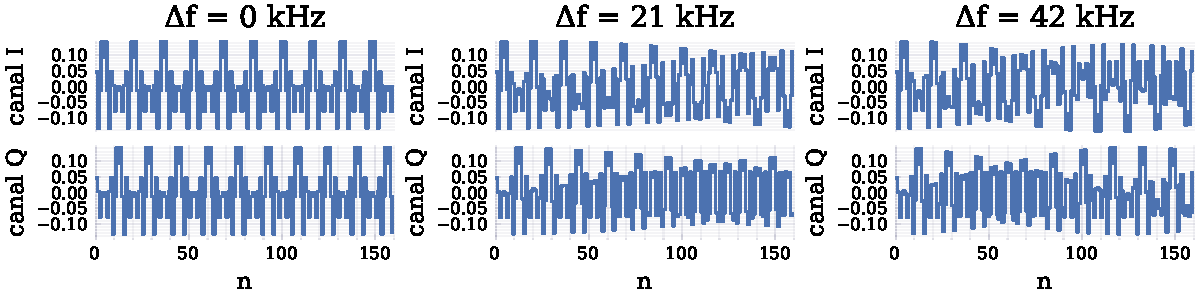
\includegraphics[width=\imsizeL]{references.pdf}
    \caption{Secuencia de entrenamiento de símbolos cortos en el dominio temporal.\label{fig:references}}  
\end{figure}


Esto permite una extensión vectorial del estimador $\Phi$, asignándole un nombre oficial de $\Phi_{BC}$ de la siguiente forma.
\begin{equation}\label{eq:correladores-banco}
    \Phi_{BC}[n,m] = \left\lvert \sum_{k=1}^{N}y^\ast[n-k]s_m[N-k] \right\rvert
\end{equation}

El resultado de aplicar el estimador a la señal entrante se representa en la figura \ref{fig:banco-xcorrN}.

\begin{figure}[ht]
    \centering{}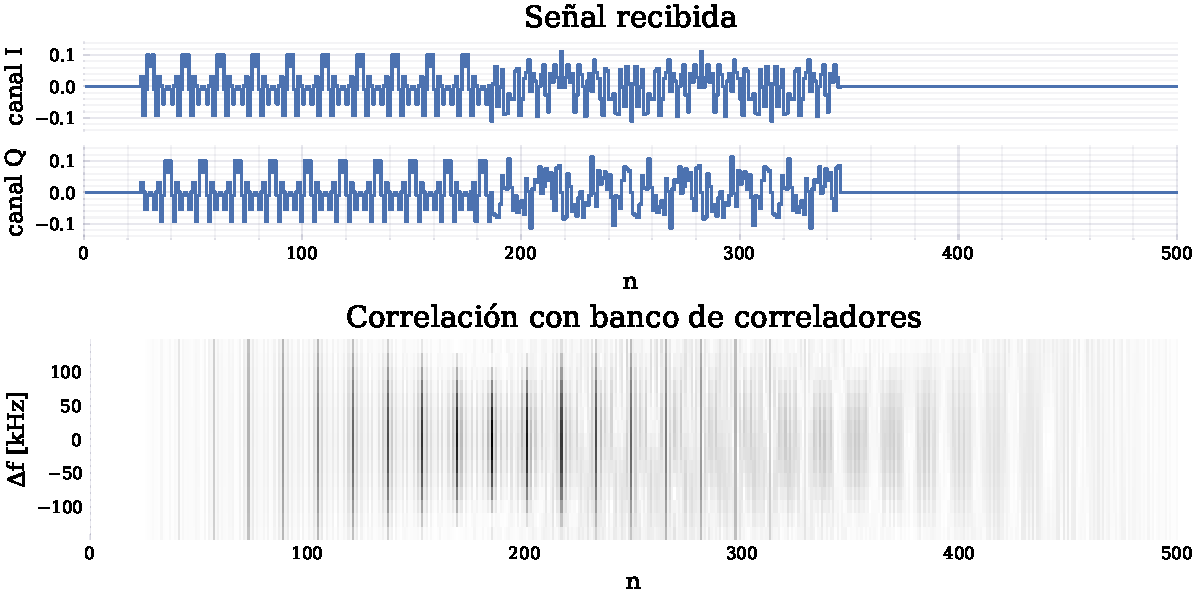
\includegraphics[width=\imsizeL]{banco-xcorrN.pdf}
    \caption{Secuencia de entrenamiento de símbolos cortos en el dominio temporal.\label{fig:banco-xcorrN}}  
\end{figure}

Se observa que $\Phi_{BC}$ definido en la ecuación \ref{eq:correladores-banco} será máximo cuando $n$ corresponda al instante en el que termina la secuencia de entrenamiento de símbolos cortos, y $m$ corresponda al íncice de referencia con error en frecuencia más cercano al error de frecuencia en recepción, permitiendo así sincronizar tanto en tiempo como en frecuencia.

\subsection{Implementación en LabVIEW}
\label{Ss:ch3-banco-labview}

\section{Método \textit{Delay and Correlate}}
\label{S:ch3-dac}

\subsection{Principio del Método}
\label{Ss:ch3-dac-principio}

El método \textit{Delay and Correlate}, a diferencia del banco de correladores, no usa la forma de onda de la secuencia de entrenamiento de símbolos cortos para sincronizar, pero si utiliza el conocimiento de su periodicidad. En su versión más simple este método se basa en identificar una señal periódica de la longitud de la secuencia de entrenamiento en la señal entrante a través del estimador $\Phi_{DC}$.

\begin{equation}
    \Phi_{DC}[n] = \sum_{k=0}^{L}y^\ast[n-k]y[n-k-L]
\end{equation}

\subsection{Implementación en LabVIEW}
\label{Ss:ch3-dac-labview}


%%% Local Variables: 
%%% mode: latex
%%% TeX-master: "template"
%%% End: 
